\chapter{Optimisation d'une ressource dans un problème de jobshop}
Cette fois ci, nous allons nous concentrer sur la modélisation d'un problème à base de \emph{jobshop} dans lequel nous étudierons le travail entre deux machines $M_1$ et $M_2$ sur deux pièces $A$ et $B$. Dans un premier temps, nous modéliserons comme dans le chapitre précédent, le GET associé à notre système. Puis nous étudierons chaque marquage initial de notre graphe, selon les ordonnancement possible, afin de déterminer le cycle de temps associé de chacun.

\section{Étude du problème}
%% Ordonnancement 1	:		M2 --> A		B
%%							M1 -->   A - B

%% Ordonnancement 2	:		M2 -->   B - A		NON RESPECT
%%							M1 -->   A - B		NON RESPECT

%% Ordonnancement 3	:		M2 --> 	 A - B
%%							M1 --> 	 B - A

%% Ordonnancement 4	:		M2 --> 	  B	- A
%%							M1 --> B 		A
Le problème de cet exercice peut être décomposé en deux sous problèmes équivalents. Le premier concerne l'ordre dans lequel les pièces $A$ et $B$ peuvent être traités par les machines : $A$ ne peut pas passer sur $M_1$ tant qu'elle n'est pas d'abord passer sur $M_2$. Pour la pièce $B$, elle doit d'abord passer par $M_1$ puis elle va sur $M_2$, comme cela est expliqué dans l'ennoncé. 

Le deuxième problème qui apparait n'en ai pas vraiment un, il s'agit de choisir l'ordonnancement des usinages de pièces. Très naturellement, pour 2 machines et 2 pièces il vient $2\times 2$ possibilité d'ordonnancement qui sont : \begin{enumerate}
\item \label{item:o1}\textbf{Ordonnancement 1} $M_2 \rightarrow A$ puis $M_1 \rightarrow A \rightarrow B$ et  $M_2 \rightarrow B$ 
\item \label{item:o2}\textbf{Ordonnancement 2} $M_2 \rightarrow B \rightarrow A $ parallèle à $M1 \rightarrow A \rightarrow B$
\item \label{item:o3}\textbf{Ordonnancement 3}	$M_2 \rightarrow A \rightarrow B $ parallèle à $M1 \rightarrow B \rightarrow A$
\item \label{item:o4}\textbf{Ordonnancement 4}	$M_1 \rightarrow B$ puis $M_2 \rightarrow A \rightarrow B$ etpour   $M_1 \rightarrow B$
\end{enumerate}

Pour modéliser notre problème sous forme de GET, nous aurons besoin des évènements qui lient les machines et les pièces entre elles. Nous pouvons obtenir ces informations à partir du tableau donné dans le sujet de TP,  Ces temps d'attentes seront utilisés dans les temps d'attentes des places du GET pour modéliser le temps que met une pièce à être usiné par une machine. L'entrée d'un jeton dans une place signifie le début du traitement d'une pièce par une machine, la fin de traitement est modélisé par la fin de l'attente d'un jeton dans une place. 

Les événements qui lient les machines aux pièces sont donc les les liaisons $A$ entre dans $M_1$, $B$ entre dans $M_1$, $A$ entre dans $M_2$ et $B$ entre dans $M_2$. Nous nous intéressons qu'aux entrés dans les machines car ce sont les événements les plus importants dans un système industriel. En effet les sortie dépendent des temps de traitement et des temps d'entrée : temps de sortie = temps de l'entrée + temps de traitement.

\section{Modélisation des GET et représentation d'état et analyse du cycle associé}

Dans un premier temps, nous avons réalisé le graphe des événements temporisés général(voir figure \ref{fig:get}). Ce graph a 4 transitions (en noir) qui se retrouvent sur les intersections entre une pièce et une machine qui doit usiner la pièce. Elles correspondent, en partant de celle en haut à gauche et dans le sens horaire, à \emph{A entre dans M1}, \emph{B entre dans M1}, \emph{B entre dans M2} et à \emph{A entre dans M2}. 

Les annotations \emph{A}, \emph{B}, \emph{M1} et \emph{M2} ne font pas partis du graph, elles font offices de légendes pour la couleurs des éléments du graph.

\begin{figure}[!ht]
\centering
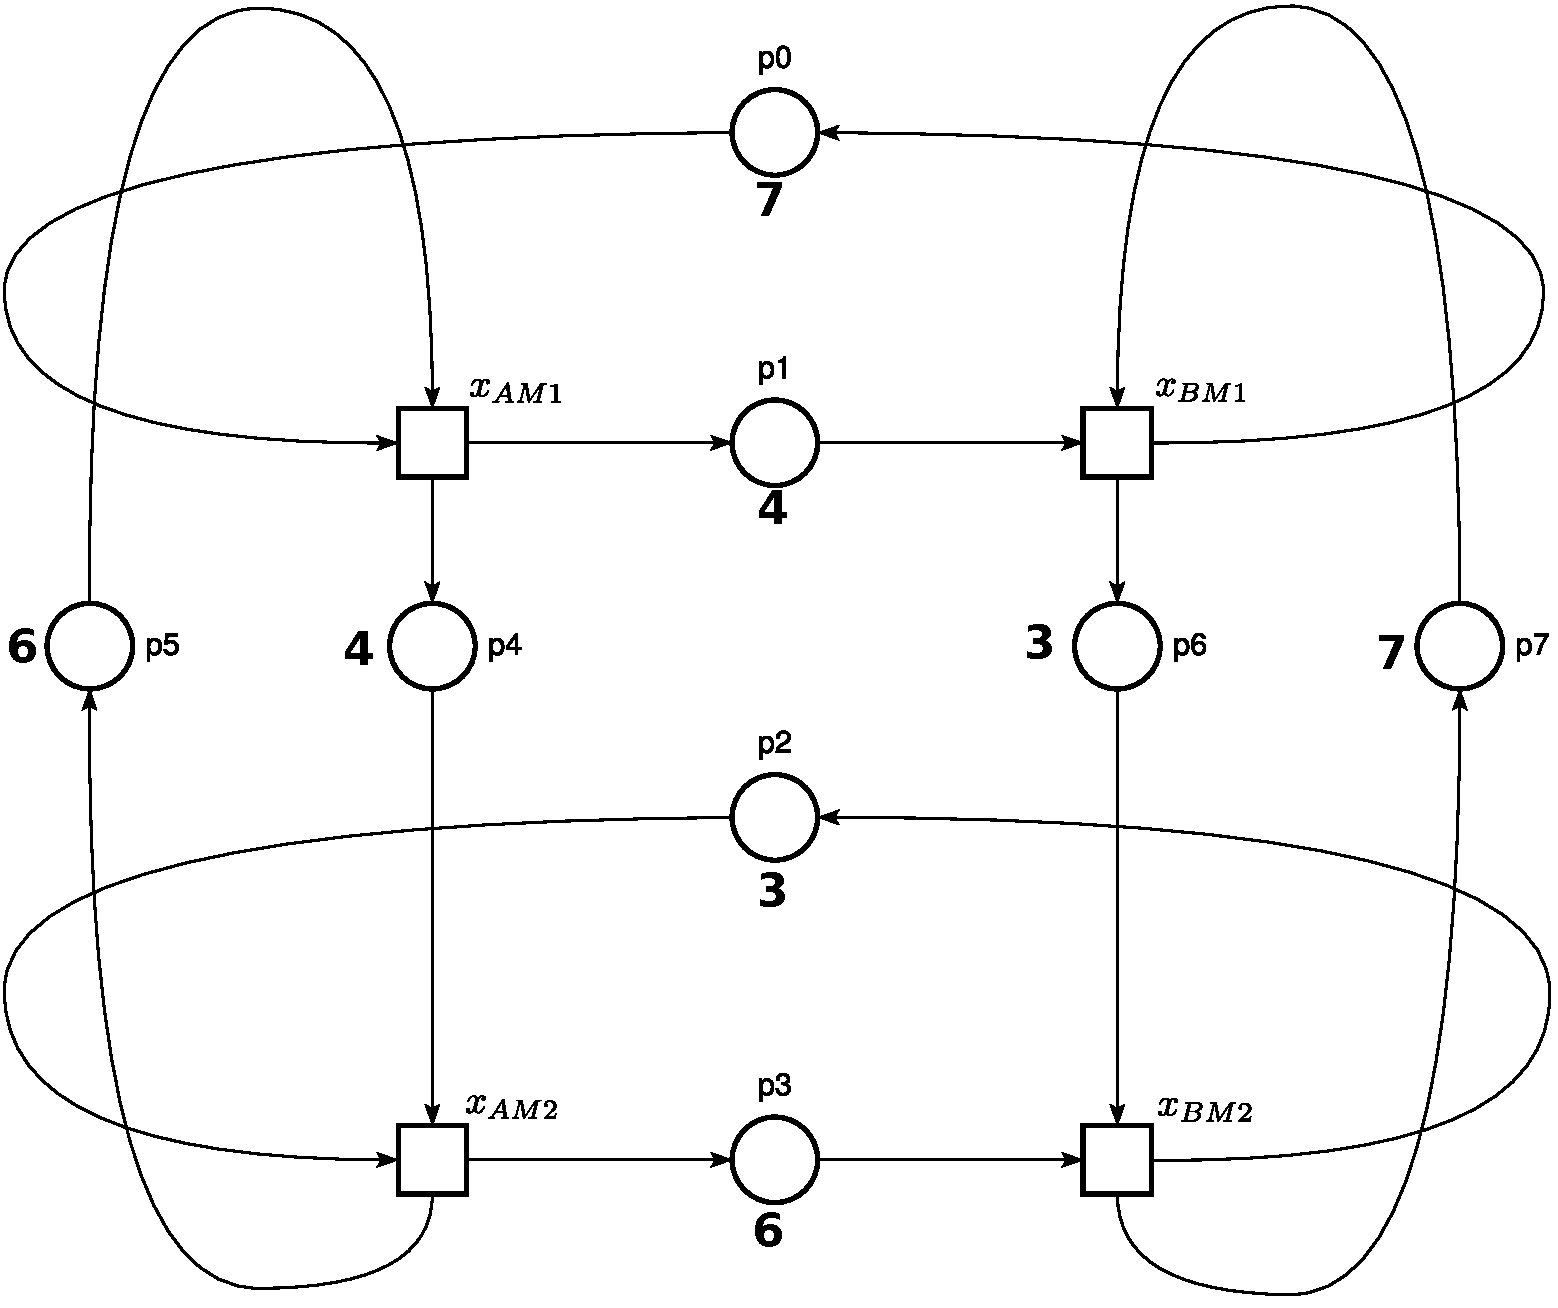
\includegraphics[width = .75\textwidth]{./II/images/GET.pdf}
\caption{\label{fig:get} Graphe des Événements Temporisé du \emph{jobshop}}
\end{figure}

Pour continuer l'analyse du système et prouver son fonctionnement, nous allons modéliser les 4 ordonnancement possible. A partir des modèles obtenu, nous étudierons avec l'algèbre (max,+) les temps de cycle maximum. Nous effectuerons les calculs grâce à l'outil informatique \emph{ScicosLab}.

La modélisation des 4 ordonnancements doit donc permettre au système d'effectuer une liste d'action bien précise. Pour cela, nous avons à notre disposition le placement de 4 jetons, car chaque élément du système, qu'il soit une pièce ou une machine, possède un jetons pour indiquer dans quelle position il se trouve.
\subsection{Ordonnancement 1}\label{sub:ordo1}
Nous modélisons maintenant le cas du premier ordonnancement possible décrit rapidement en \ref{item:o1}. Dans ce cycle, la pièce $A$ doit d'abord passer sur la machine $M_2$ puis prendre la machine $M_1$. Ensuite c'est au tour de la pièce $B$ de prendre les machines $M_1$ puis $M_2$. 

Pour que la pièce $A$ occupe la première utilisation de $M_2$, nous devons placer le marquage initial dans les places $p4$ et $p2$ pour sensibiliser la transition $x_{AM2}$ et ainsi modéliser l'entrer de $A$ dans la machine 2. On souhaite aussi que $A$ utilise la machine 1 avant $B$, donc on empêche la sensibilisation de $x_{BM1}$ en ne mettant pas de jeton dans la place $p1$ mais en plaçant un jeton dans la place $p0$. Pour que la pièce $B$ commence par la machine $M_1$, i.e $x_{BM1}$, nous plaçons un jeton dans la place $p7$. 

Nous obtenons la figure suivante (\ref{fig:get1}). Avec l'outil \emph{Stepper Simulator} disponible grâce à TINA, nous avons été capables de simuler notre modèle pour vérifier l'ordonnancement.
\begin{figure}
\begin{center}
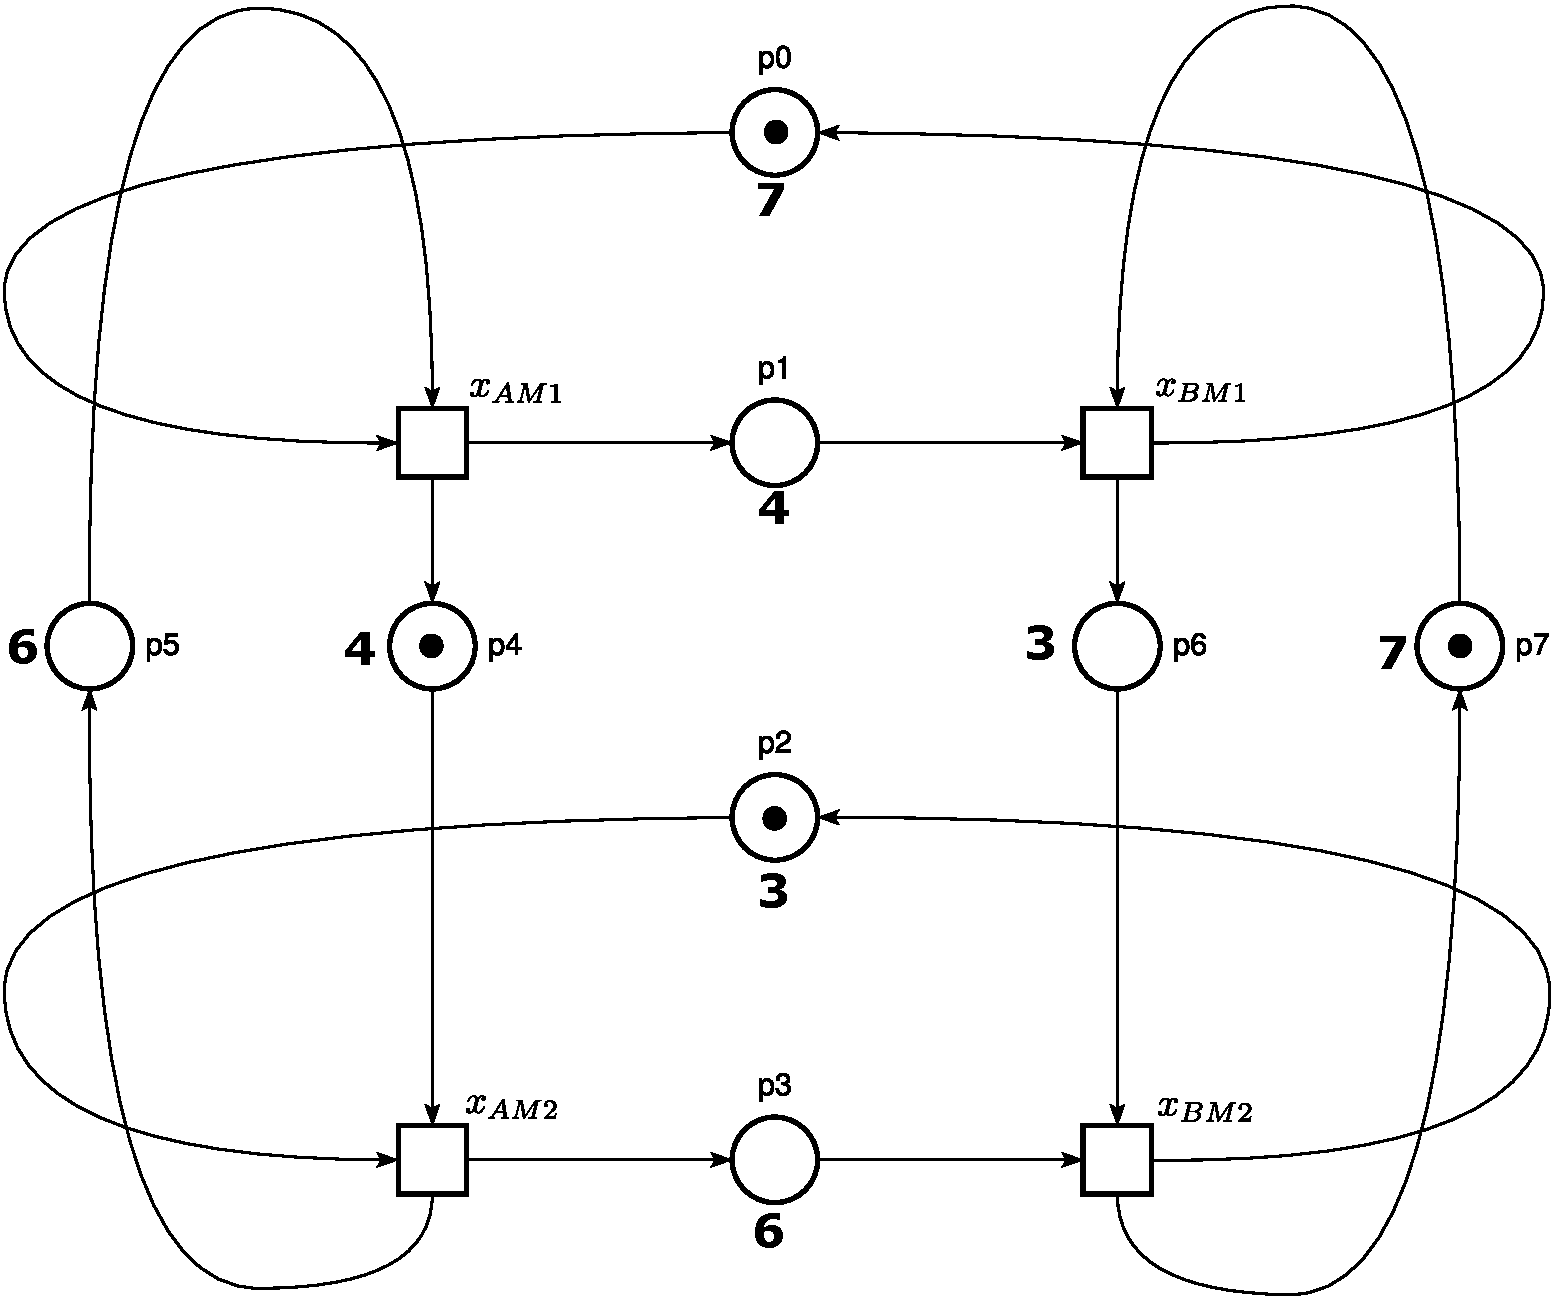
\includegraphics[width = .75\textwidth]{./II/images/GET_1.pdf}
\captionof{figure}{\label{fig:get1} Graphe des Événements Temporisé de l'ordonnancement 1 (\ref{item:o1})}
\end{center}
\end{figure}
 
Nous souhaitons analyser le GET obtenu pour connaitre si celui ci est optimal. Nous devons donc commencer par écrire les équations qui décrivent notre système :  
\begin{align*}
&\left\lbrace
\begin{array}{lcl}
x_{AM_1}(k)&=&  6x_{AM_2}(k) \oplus 7x_{BM_1}(k-1)\\
x_{AM_2}(k)&=&4x_{AM_1}(k-1) \oplus 3x_{BM_2}(k-1)\\
x_{BM_1}(k)&=& 4x_{AM_1}(k) \oplus 7x_{BM_2}(k-1)\\
x_{BM_2}(k)&=& 6x_{AM_2}(k) \oplus 3x_{BM_1}(k)\\
\end{array}
\right.\\
&\Leftrightarrow \begin{pmatrix}
x_{AM_1}(k)\\
x_{AM_2}(k)\\
x_{BM_1}(k)\\
x_{BM_2}(k)
\end{pmatrix} = \begin{pmatrix}
. & 6 & . & .\\
. & . & . & .\\
4 & . & . & .\\
. & 6 & 3 & .\\
\end{pmatrix} \begin{pmatrix}
x_{AM_1}(k)\\
x_{AM_2}(k)\\
x_{BM_1}(k)\\
x_{BM_2}(k)
\end{pmatrix} \oplus \begin{pmatrix}
. & . & 7 & .\\
4 & . & . & 3\\
. & . & . & 7\\
. & . & . & .\\
\end{pmatrix} \begin{pmatrix}
x_{AM_1}(k-1)\\
x_{AM_2}(k-1)\\
x_{BM_1}(k-1)\\
x_{BM_2}(k-1)
\end{pmatrix}
\end{align*}
Ce système d'équation n'est pas utilisable tel quel, nous allons continuer la factorisation pour obtenir une forme du type :$X(k)=f(X(k-1))$. Finalement, il vient en insérant les éléments en $k-1$ dans les éléments en $k$ : 
\begin{align*}
\left\lbrace
\begin{array}{lcl}
x_{AM_1}(k)&=& 10x_{AM_1}(k-1) \oplus 9x_{BM_2}(k-1)\oplus 7x_{BM_1}(k-1)\\
x_{AM_2}(k)&=&4x_{AM_1}(k-1) \oplus 3x_{BM_2}(k-1)\\
x_{BM_1}(k)&=& 11x_{BM_1}(k-1) \oplus 14x_{AM_1}(k-1) \oplus 13x_{BM_2}(k-1)\\
x_{BM_2}(k)&=& 20x_{BM_2}(k-1) \oplus 21x_{AM_1}(k-1) \oplus 18x_{BM_1}(k-1)\\
\end{array}
\right.
\end{align*}
d'où :
\begin{align}\label{equ:ordo1}
X(k) = \begin{pmatrix}
x_{AM1}(k) \\ x_{AM2}(k) \\ x_{BM1}(k)\\ x_{BM2}(k)
\end{pmatrix} 
= \begin{pmatrix}
10 & . & 7 &9\\
4 & . & . & 3\\
14 & . & 11 & 13\\
21 & . & 18 & 20
\end{pmatrix}X(k-1) = A_1X(k-1)
\end{align}
Il est maintenant possible d'étudier le temps de cycle de notre système grâce à l'algèbre (max,+) avec le calcul de la ou les valeur(s) propres. Nous ne sommes pas déterministe sur le nombre de valeurs propres de la matrice d'évolution car ce système n'est pas irréductible. Nous obtenons avec \emph{ScicosLab} et la fonction \emph{karp} le résultat suivant : \begin{eqnarray*}
\lambda(A_1) = 20
\end{eqnarray*}
Ce temps de cycle maximal correspond à la somme des temps de traitement de toute les machines. Il était possible de prévoir ce résultat car l'ordonnancement n'est pas optimal, les machines passent du temps en étant inactive. Nous verrons qu'un meilleur ordonnancement est possible dans la suite de ce rapport.

\subsection{Ordonnancement 2}
L'ordonnancement 2 n'est pas réalisable. En effet, il n'est pas compatible avec la spécification sur l'ordre dans lequel les pièces $A$ et $B$ doivent être usiné par les machines. Nous n'avons alors pas pu dessiner le GET associé.

\subsection{Ordonnancement 3}
Nous allons effectuer la même analyse que dans la partie précédente (\ref{sub:ordo1}). Dans cette répartition des traitement de pièces, nous allons synchroniser l'usinage de la pièce $A$ par $M_2$ et de $B$ par $M_1$ puis l'inverse ($A$ par $M_1$ et $B$ par $M_2$). 

Pour obtenir cette séquence, il est nécessaire de disposer le marquage initial de sorte à ce que $x_{AM2}$ et $x_{BM1}$ soit sensibiliser dès le début du traitement.
\begin{figure}[!ht]
\centering
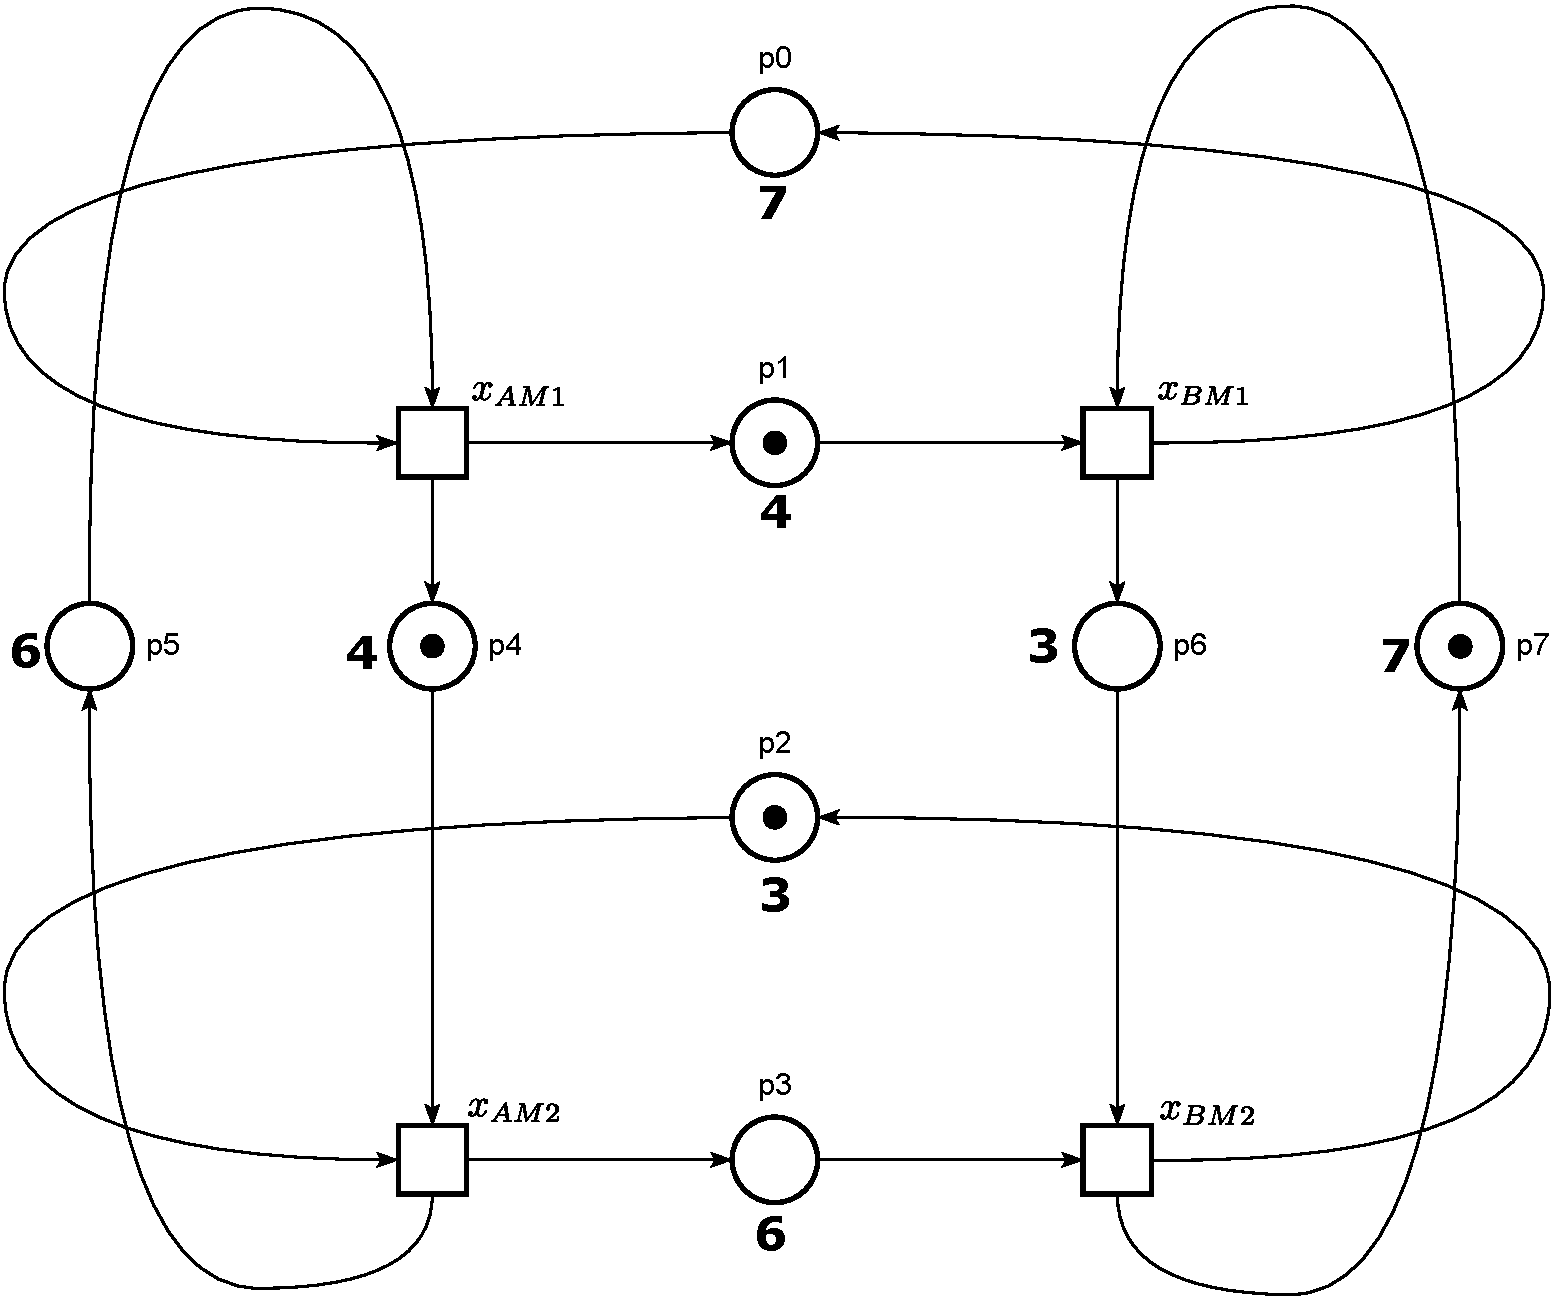
\includegraphics[width = .75\textwidth]{./II/images/GET_3.pdf}
\caption{\label{fig:get} Graphe des Événements Temporisé de l'ordonnancement 3 (\ref{item:o3})}
\end{figure}

Nous pouvons écrire le système d'équation du GET obtenu que nous vous présentons ci dessous. Nous avons effectué une étape avant l'écriture de ce système, en écrivant le système sous la forme $X(k)=f(X(k),X(k-1))$ :
\begin{align*}%\label{equ:ordo3}
\left\lbrace
\begin{array}{lcl}
x_{AM_1}(k)&=& 10x_{AM_1}(k-1) \oplus  9x_{BM_2}(k-1)\\
x_{AM_2}(k)&=&  4x_{AM_1}(k-1) \oplus  3x_{BM_2}(k-1)\\
x_{BM_1}(k)&=&  4x_{AM_1}(k-1) \oplus  3x_{BM_2}(k-1)\\
x_{BM_2}(k)&=& 10x_{BM_2}(k-1) \oplus 11x_{AM_1}(k-1)\\
\end{array}
\right.
\end{align*}
Ce système d'équation du GET peut être représenté sous forme espace d'état avec le même vecteur que d'état que dans \ref{equ:ordo1}. Nous obtenons :
\begin{align}\label{eqn:eeOrdo3}
X(k) = \begin{pmatrix}
10 & . &. & 9\\
4 &. &. & 3\\
4 &. &. & 3\\
11 &. &. & 10\\
\end{pmatrix}X(k-1) = A_2X(k-1)
\end{align} 
Comme pour l'ordonnancement précédent, nous calculons la valeurs propres du système pour le temps de cycle : 
\begin{eqnarray*}
\lambda(A_2) = 11  
\end{eqnarray*}
Ce cycle maximal correspond à l'usinage de la machine $M_1$ pour les deux pièces. Il s'agit du cycle le plus long, cycle de $A$ = cycle de $B$ = 10 et le cycle de $M_2$ = 9. Cet ordonnancement est le plus optimal, $M_1$ ne va jamais s'arrêter car c'est elle même qui ralentir le système. 
\subsection{Ordonnancement 4}
Cette mise en place des usinages est l'opposé de l'ordonnancement 1. Nous avons ici la pièce $B$ qui doit passer sur $M_1$ puis $M_2$, ce qui débloquera $A$ pour qu'elle puisse être traité par $M_2$ puis $M_1$. Les 4 jetons que nous décidons de placer sont visibles sur la figure \ref{fig:get4}.
\begin{figure}[!ht]
\centering
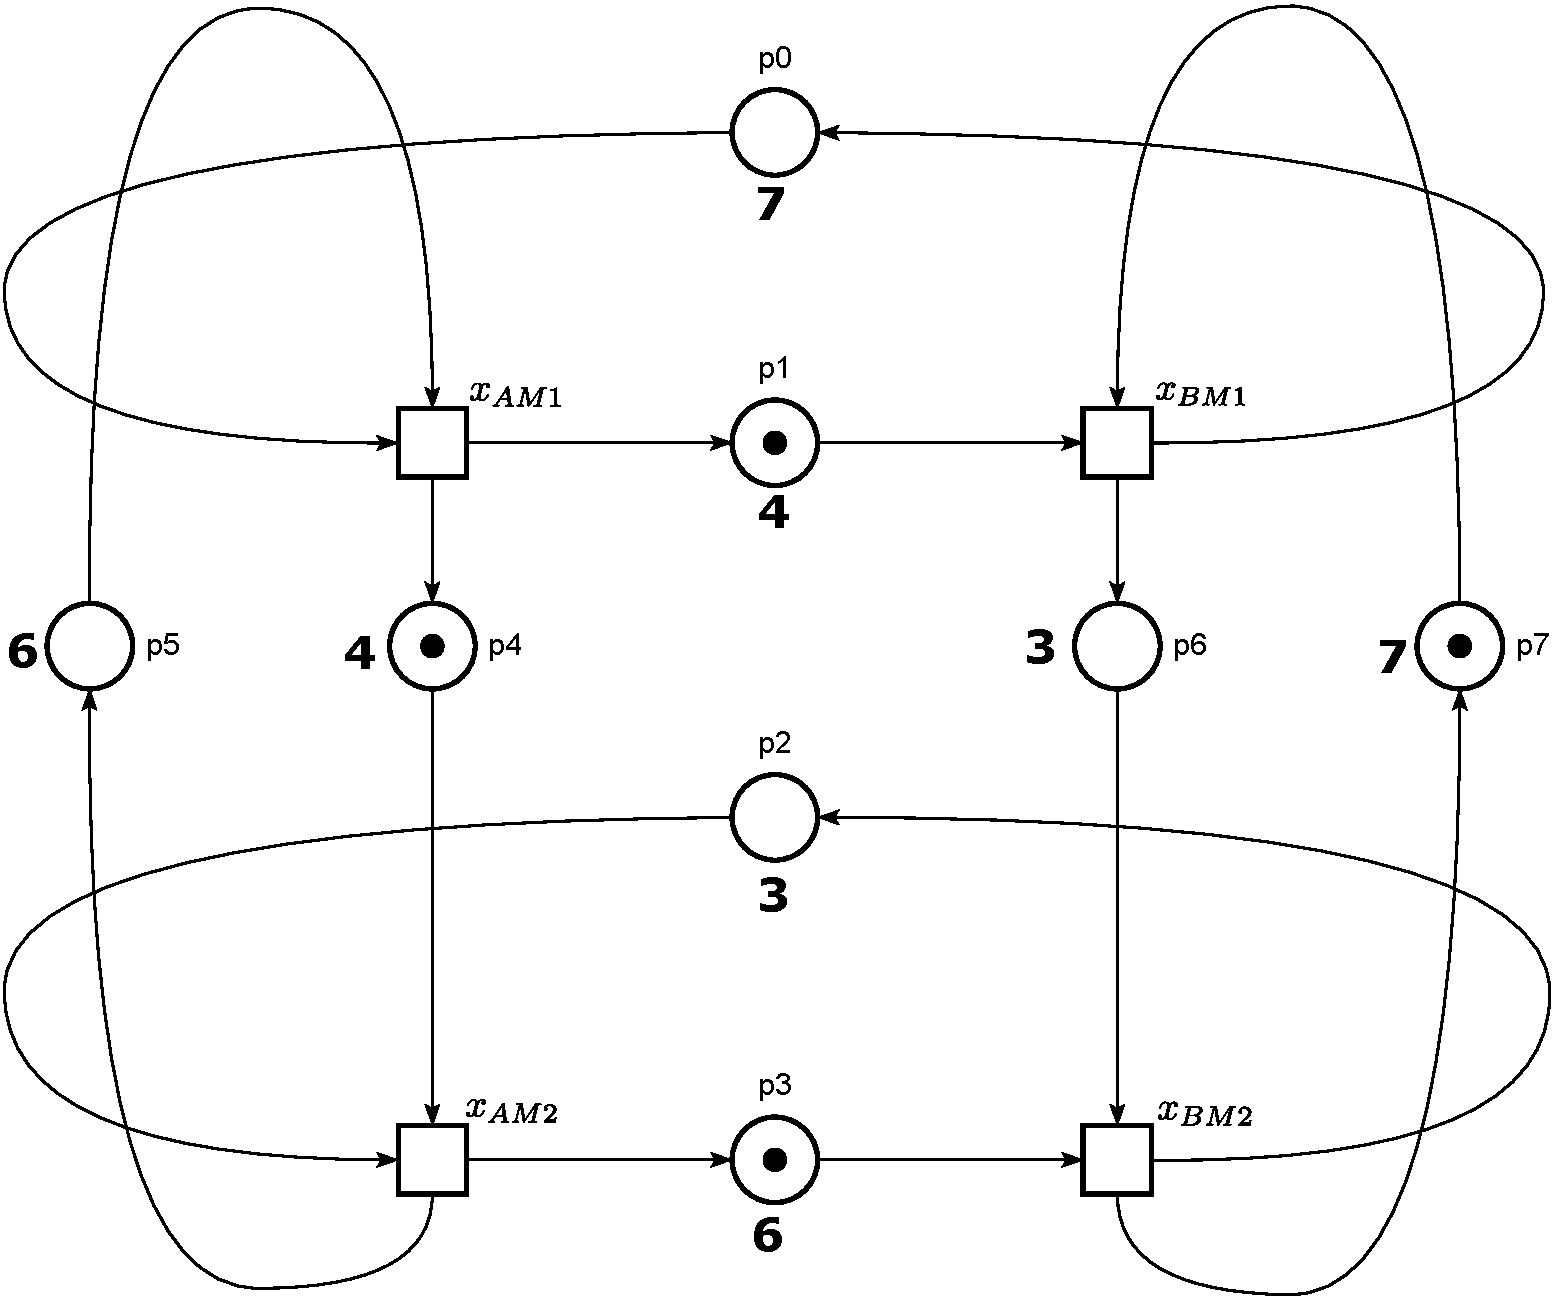
\includegraphics[width = .75\textwidth]{./II/images/GET_4.pdf}
\caption{\label{fig:get4} Graphe des Événements Temporisé de l'ordonnancement 4(\ref{item:o4})}
\end{figure}

Les calculs pour obtenir le système d'équation du GET ne sont pas détaillé ici. Nous obtenons : 
\begin{align*}%\label{equ:ordo4}
\left\lbrace
\begin{array}{lcl}
x_{AM_1}(k)&=& 20x_{AM_1}(k-1) \oplus 19x_{BM_2}(k-1) \oplus 15x_{AM2}(k-1)\\
x_{AM_2}(k)&=& 14x_{AM_1}(k-1) \oplus 13x_{BM_2}(k-1) \oplus  9x_{AM2}(k-1)\\
x_{BM_1}(k)&=&  4x_{AM_1}(k-1) \oplus  3x_{BM_2}(k-1)\\
x_{BM_2}(k)&=& 10x_{BM_2}(k-1) \oplus 11x_{AM_1}(k-1) \oplus  6x_{AM2}(k-1)\\
\end{array}
\right.
\end{align*}
qui revient à écrire en forme d'état : 
\begin{align}\label{eqn::ee_Ordo4}
X(k) = \begin{pmatrix}
20 & 15 & . & 19\\
14 & 8  & . & 13\\
4  & .  & . & 3 \\
11 & 6  & . & 10
\end{pmatrix}X(k-1) = A_4X(k-1)
\end{align}

Avec la matrice d'évolution donné en \ref{eqn::ee_Ordo4}, nous pouvons établir le temps de cycle maximum comme dans les ordonnancement 1 et 3 avec la valeur de la valeur propre :
\begin{equation}
\lambda(A_4) = 20
\end{equation}

Comme dans l'ordonnancement étudié en \ref{sub:ordo1}, nous trouvé une valeur propres élevé qui correspond encore une fois à la somme du temps de traitement de toute les machines et cess pour la même raison évoqué dans la première étude.

\section{Synthèse}
Nous avons été capable grâce aux Graphes d'évènements temporisé de mettre en place une étude des différents ordonnancement. Nous avons remarqué qu'il est possible de tomber sur des cas impossible car ils ne respectent pas les conditions de bon fonctionnement. Il existe aussi des ordonnancement qui sont meilleurs que d'autres, comme nous l'avons observé entre le n°1 et le n°2. Grâce à l'algèbre (max,+), nous avons même été capables de prouver que l'ordonnancement 2 est meilleur que les autres et qu'il utilise au mieux les ressources qui lui sont à disposition. 